
\documentclass[sigconf,nonacm]{acmart}

\AtBeginDocument{%
  \providecommand\BibTeX{{%
    \normalfont B\kern-0.5em{\scshape i\kern-0.25em b}\kern-0.8em\TeX}}}

\begin{document}

%%
%% The "title" command has an optional parameter,
%% allowing the author to define a "short title" to be used in page headers.
\title{Spotify recommender}
\subtitle{Fundamenten van Mens-machine interactie [G0Q55a]}

\author{ABC DEFGH}
\email{r123456}

\author{ABC DEFGH}
\email{r123456}

\author{ABC DEFGH}
\email{r123456}

\author{Dries Vuylsteke}
\email{r0712986}

\renewcommand{\shortauthors}{Group X}

%%
%% The abstract is a short summary of the work to be presented in the
%% article.
\begin{abstract}
  An analysis of how familiarity in song suggestions are related to the confidence in the provided suggestions. This paper takes a closer look at how familiarity interferes with confidence in a recommendation. A music recommender system was developed by first making a paper prototype and using this to do a think aloud study. The prototype design was changed based on the data gathered from this first study. A digital implementation was made, which was then put to another think aloud test. Again the data was used to make the interface more user friendly.
  Finally a a study was conducted to examine the relationship of user confidence and the familiarity of the recommended music. The expected results are that the result would be counterintuitive. When looking for new music you expect unknown results, yet familiar results might give you more confidence that the program works.
  TODO: research conclusion
\end{abstract}


\begin{teaserfigure}
  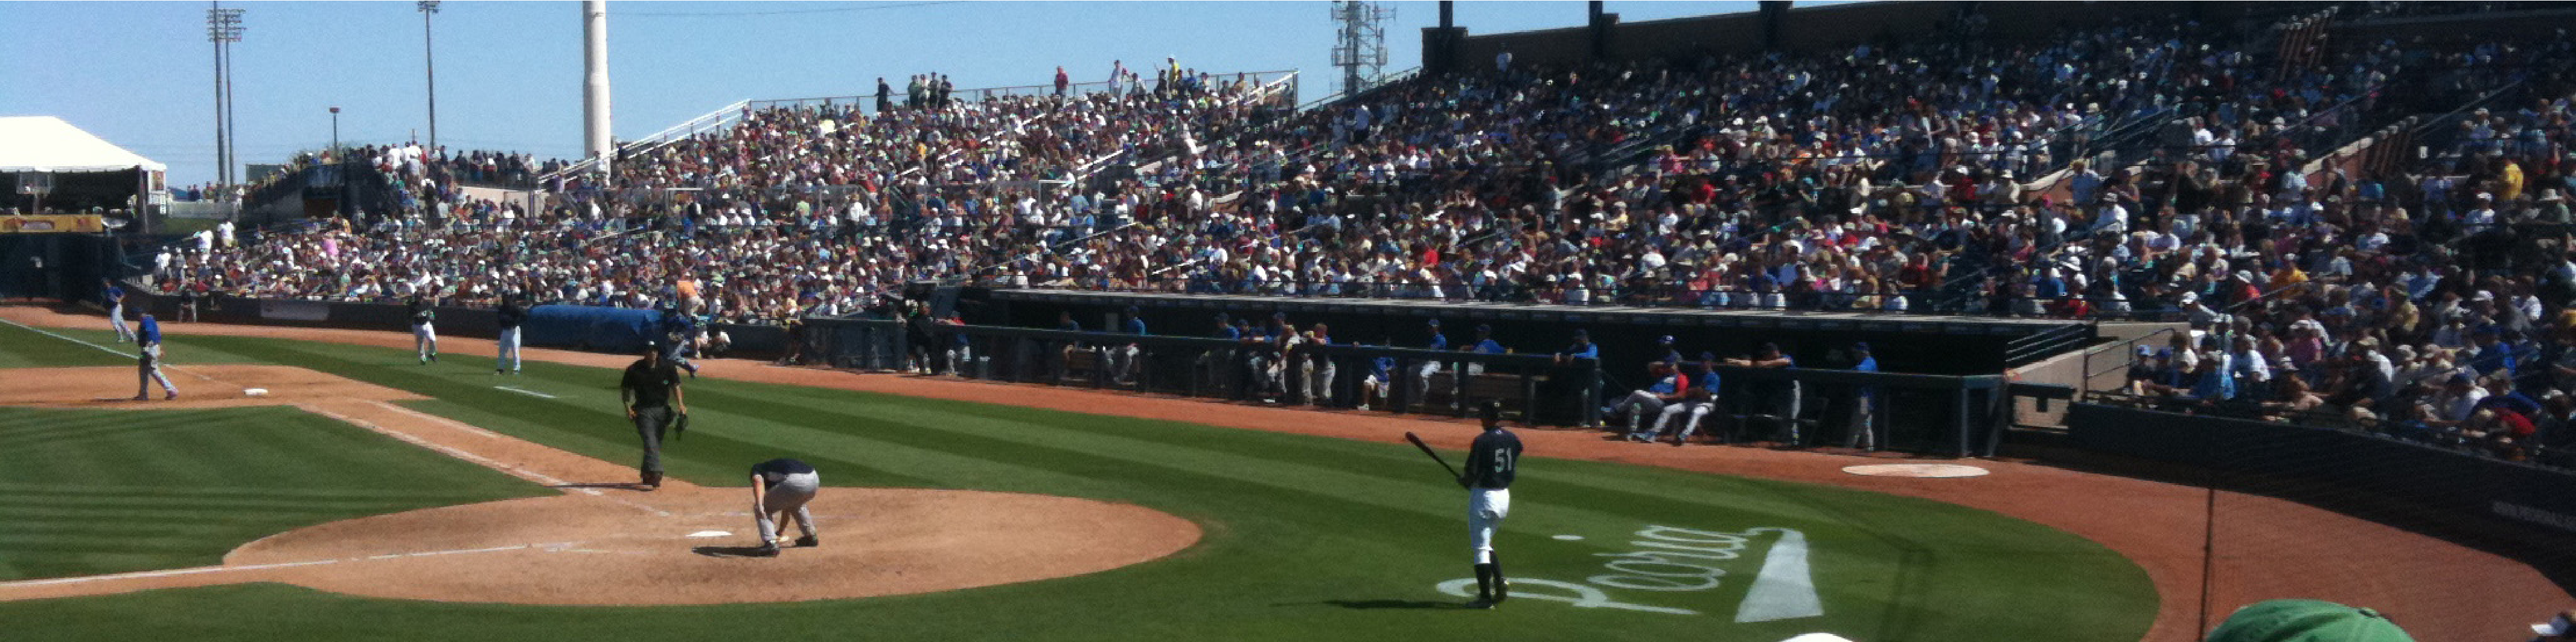
\includegraphics[width=\textwidth]{sampleteaser}
  \caption{Insert spotify recommender icon here}
  \Description{Enjoying the baseball game from the third-base
  seats. Ichiro Suzuki preparing to bat.}
  \label{fig:teaser}
\end{teaserfigure}

%%
%% This command processes the author and affiliation and title
%% information and builds the first part of the formatted document.
\maketitle




\section{Introduction}
The internet is filled with recommender systems. Think of Facebooks "you might like this" posts on your timeline, Netflix's home page filled with recommendations and spotify giving you daily playlists filled with songs they think you might like. While all these recommendations make life easier, they are usually hidden behind a black box algorithm. The result is that users do not understand why certain recommendations pop up for them and as a result their trust in the applications recommendations is lowered. For third party developers that use the API of an existing system this isue becomes even worse. Applications like youtube grant user trust because they are well known to be working well. Third party variants that suggest video's are probably not as well trusted.

In an attempt to give the user more trust in the system, a good user interface can be designed. User experience and user interface design are closely linked, this much has been determined [TODO: source??]. Now to take this prospect further: while looking for something new by using a recommender engine, does seeing something familiar increase trust in the unknown? Because users are not familiar with the internal workings of a system, does it increase trust if they see some suggestions they know to be good?

This paper was written based on the results from following the course Fundamenten van de Mens-machine interacite [G0Q55a] at KU Leuven University. This course aims to give knowledge about human-computer interaction and how it can be applied to develop user-friendly applications.

In this paper the approach towards designing a music recommender user interface based on the spotify API is described. The prototype is built based on feedback from the target audience, gained through think aloud studies. Once the application was made, a study was performed to see if the users had more trust in recommendations that were considered to be more popular (and therefore familiar).

The posed research questions were the following:
1: Does the popularity of the given suggestions affect the trust of users in the application?
2: Does the popularity of the given suggestions affect how many recommendations are interacted with?
3..

The remainder of the paper is structured as followed: first some related work is cited to give the reader a chance for more in depth reading. Then in section three the implementation of the application is provided. This ranges from the used recommender system, to the interface design. In section four this is followed up with the experiment. Some information is given about the participants, how the study was performed and how the measurements were taken. Finally the last two chapters contain the results of the experiment in section five and some discussion about the results in section six. The paper is wrapped up with a conclusion about the posed research questions.

\begin{itemize}
    \item What is the problem and the context?
    \item Why is the problem relevant?
    \item How do we solve this problem?
    \item What are the research questions?
\end{itemize}

\section{Related work}
The internet is filled with third-party applications to help spotify users make better playlists and help them get to know new music. Examples range from github distributions [https://github.com/mrthlinh/Spotify-Playlist-Recommender] to websites [https://magicplaylist.co/].

The inspiration for this projects was found during the lectures of the  course for which the project was developed. One of the lecturers had done research based around trust in the spotify recommender [Controlling Spotify recommendations: effects of personal characteristics on music recommender user Interfaces]. The power of the spotify API shown in this research proned our team to make a similar application for our course.

\begin{itemize}
    \item Which similar applications exist?
    \item Where did you get some inspiration?
    \item [optional] Which papers did you read and how do they relate to your work?
\end{itemize}

\section{Implementation}
\subsection{Data}
see next section
\begin{itemize}
    \item Which data did you use?
    \item Where did you find it?
    \item Was there a need for filtering the data?
\end{itemize}

\subsection{Recommender system}
The recommender algorithm used in this project is the official Spotify recommender exposed through the spotify API. This algorithm is a black box approach towards recommendations, which means it was perfect for the posed research question. 
The original choice was made purely because of curiosity towards the possibilities of the API. The original recommendations spotify provide easily become lackluster for the regular user. The API exposes several extra parameters to the users, allowing for far more specific recommendations.
\begin{itemize}
    \item Which recommender algorithm did you use?
    \item Why?
    \item Which program did you use?
\end{itemize}

\subsection{Interface}
The application first allows you to pick an existing playlist and select some seed songs from it. It then analyses those songs and gives you the possiblity to change certain properties of the recommendations that will be given. The final screen, and the important one for this application gives several tracks based on the selected playlist, songs, and adjusted music properties. The user has the possibility to listen to each suggestion individually to see if they like the suggestions. Once the user is satisfied with the quality of the suggestions he can either add them to the originally selected playlist, or save them to a new playlist.

The interface was implemented iteratively based on think aloud studies, each time performed on different users. The initial prototype was a paper prototype made with the idea to just generate an entire playlist based on the original playlist, and the adjusted music properties. It contained three screens: a playlist selection, a value tweaker and a result page. We then digitalised this prototype with [TODO: INSERT PROTOTYPE APP???] and performed a think-aloud study. 

The results of the think aloud study and the original paper prototype were used to make the digital prototype. The first iteration of the digital prototype was designed using Unity, but was quickly replaced with Ionic as it became clear that Unity would make the design process a lot harder than it needed to be. The further implementation of the digital prototype was done using Ionic, a JavaScript framework. Once this was fully functional an additional think aloud study was performed to optimise the user interface.

TODO: expand upon the framework specs

\begin{itemize}
    \item What does the interface look like? (Discuss only the most important 1 or 2 screens, other screenshots belong in the appendix).
    \item How did you implement the interface methodologically (How did you involve user, how many iterations before the final study)
    \item How did you implement the interface technically (Which framework/library/language/etc )
\end{itemize}

\section{Experiment}
\subsection{Participants}
\begin{itemize}
    \item How many participants?
    \item How did you recruit them?
    \item Characteristics (gender, age, background).
\end{itemize}

\subsection{Experimental design}
\begin{itemize}
    \item AB or within?
    \item Lab study or in the wild?
    \item Flow of the study (e.g. install-test-task1-evaluation1-task2-evaluation2-final evaluation).
    \item Reasoning behind this design.
\end{itemize}

\subsection{Measurements}
\begin{itemize}
    \item Which questions did you ask?
    \item Which interactions did you log?
    \item What was the goal to log/ask these?
\end{itemize}

\section{Results}
\subsection{Statistics}
\begin{itemize}
    \item Which data do you have? (normal, numerical/categorical, continuous/discrete)
    \item Which tests did you use?
    \item Which assumptions do this test have 
\end{itemize}
\subsection{Quantitative results}
\begin{itemize}
    \item What are the results?
    \item Visualise the results.
\end{itemize}

\subsection{Qualitative results}
\begin{itemize}
    \item What are the results?
    \item Describe the results.
\end{itemize}

\section{Discussion}
\begin{itemize}
    \item What trends do we see?
    \item What could be the reason for these trends?
    \item What can we learn?
    \item What are the implications?
\end{itemize}

\section{Conclusion}
This is the part in which you explain to the reader what they should remember.
If most parts of the paper are about \texttt{WHAT} this part is mostly about the \texttt{SO WHAT}
\url{https://www.time4writing.com/writing-resources/writing-a-good-conclusion-paragraph/}


%%
%% The next two lines define the bibliography style to be used, and
%% the bibliography file.
\bibliographystyle{ACM-Reference-Format}
\bibliography{sample-base}
\clearpage
%%
%% If your work has an appendix, this is the place to put it.
\appendix

\section{Appendix A: Research methods}

\subsection{Part One}

Lorem ipsum dolor sit amet, consectetur adipiscing elit. Morbi
malesuada, quam in pulvinar varius, metus nunc fermentum urna, id
sollicitudin purus odio sit amet enim. Aliquam ullamcorper eu ipsum
vel mollis. Curabitur quis dictum nisl. Phasellus vel semper risus, et
lacinia dolor. Integer ultricies commodo sem nec semper.

\subsection{Part Two}

Etiam commodo feugiat nisl pulvinar pellentesque. Etiam auctor sodales
ligula, non varius nibh pulvinar semper. Suspendisse nec lectus non
ipsum convallis congue hendrerit vitae sapien. Donec at laoreet
eros. Vivamus non purus placerat, scelerisque diam eu, cursus
ante. Etiam aliquam tortor auctor efficitur mattis.

\section{Appendix B: Online resources}

Nam id fermentum dui. Suspendisse sagittis tortor a nulla mollis, in
pulvinar ex pretium. Sed interdum orci quis metus euismod, et sagittis
enim maximus. Vestibulum gravida massa ut felis suscipit
congue. Quisque mattis elit a risus ultrices commodo venenatis eget
dui. Etiam sagittis eleifend elementum.

Nam interdum magna at lectus dignissim, ac dignissim lorem
rhoncus. Maecenas eu arcu ac neque placerat aliquam. Nunc pulvinar
massa et mattis lacinia.

\end{document}
\endinput
%%
%% End of file `sample-authordraft.tex'.
